\documentclass[conference]{IEEEtran}
\usepackage{graphicx}
\usepackage{amsmath}
\usepackage{amssymb}
\usepackage{algorithm}
\usepackage{algorithmic}
\usepackage{hyperref}
\usepackage{booktabs}
\usepackage{multirow}
\usepackage{xcolor}
\usepackage{listings}
\usepackage{tikz}
\usepackage{pgfplots}
\usepackage{subcaption}
\usepackage{enumitem}
\usepackage{float}
\usepackage{balance}

\usetikzlibrary{shapes.geometric, arrows.meta, positioning, fit, calc, patterns}
\pgfplotsset{compat=1.18}

\lstset{
  basicstyle=\ttfamily\footnotesize,
  keywordstyle=\color{blue},
  commentstyle=\color{gray},
  stringstyle=\color{red},
  breaklines=true,
  frame=single,
  numbers=left,
  numberstyle=\tiny\color{gray},
  xleftmargin=2em,
  framexleftmargin=1.5em
}

\title{Blockchain-Based Audit Trails for Verifiable and Trustworthy Synthetic Data Generation}
\author{%
  \resizebox{\textwidth}{!}{%
    \begin{tabular}{cccc}
      \textbf{Abhipsa Srivastava} & \textbf{Atul Maurya} & \textbf{Abhishek Malviya} & \textbf{Harshit Mishra} \\[2pt]
      United Institute of Technology & United Institute of Technology & United Institute of Technology & United Institute of Technology \\[2pt]
      Prayagraj, India & Prayagraj, India & Prayagraj, India & Prayagraj, India \\[2pt]
      \texttt{abhipsasri8183@gmail.com} & \texttt{atulmaurya1804@gmail.com} & \texttt{abhishekmalviya@united.ac.in} & \texttt{harshit707125@gmail.com}
    \end{tabular}%
  }%
}


\begin{document}

\maketitle
\begin{abstract}
Verifying synthetic data quality in privacy-regulated environments presents a fundamental challenge: traditional evaluation methods require direct access to real data, which is precisely what regulations like GDPR and HIPAA prohibit. We present a two-layer framework that decouples verification from real-data access while producing tamper-evident, publicly auditable quality certificates.
The verification layer evaluates synthetic datasets across three dimensions without exposing source records: privacy (Distance to Closest Record, k-anonymity, and membership inference attack resistance), utility (Wasserstein distributional distance and train-on-synthetic/test-on-real ML accuracy degradation capped at 10\%), and fairness (demographic parity gap below 5\%). Multiple independent verifiers run this protocol concurrently, and their scores are aggregated via median consensus --- a choice that provides Byzantine fault tolerance for up to $\lfloor(n-1)/2\rfloor$ dishonest participants.
The blockchain layer records each verification event as an immutable transaction on Hyperledger Fabric, storing cryptographic hashes, metric summaries, and consensus proofs on-chain while keeping raw datasets off-chain in IPFS. A secondary application-level hash chain guards local logs during network unavailability. A compliance engine then maps measured scores to specific articles in GDPR, HIPAA, and the EU AI Act.
Evaluated on the UCI Adult Income benchmark (48K samples), the framework achieves 88\% agreement with full-access baselines and completes end-to-end verification --- including CTGAN generation, privacy checks, consensus, and blockchain commit --- in under 40 seconds for 10,000-row datasets. Ablation confirms each verification component contributes measurably to the composite trust score.
\end{abstract}

\begin{IEEEkeywords}
Blockchain, Synthetic Data, Privacy, Audit Trail, CTGAN, Fairness, Hyperledger Fabric, Verification
\end{IEEEkeywords}

\section{Introduction}
% Introduction

While synthetic data models like the Conditional Tabular GAN (CTGAN)~\cite{xu2019ctgan} offer a powerful workaround to strict data sharing frameworks such as GDPR~\cite{gdpr2016regulation}, HIPAA~\cite{hipaa1996act}, and the EU AI Act~\cite{euaiact2024}, proving the quality and safety of the generated data remains a fundamental challenge. Currently, a data officer runs local, isolated validation scripts and shares a self-certified quality report alongside the synthetic data. This fragile paradigm forces down-stream consumers to blindly trust the generating entity, lacking an immutable audit trail and frequently overlooking vital fairness audits~\cite{hardt2016equality}.

Distributed ledgers~\cite{nakamoto2008bitcoin} provide an avenue for tamper-proof provenance, but a blockchain cannot inherently verify the accuracy of the off-chain data being recorded---a limitation formally known as the ``oracle gap''~\cite{zheng2018blockchain}. This paper bridges that gap by cryptographically anchoring a rigorous, multi-metric objective evaluation system directly to the immutability of blockchain technology. 

To systematically explore this architecture, we structure our investigation around five central questions targeting: \textbf{Q1} (\textit{Efficacy}) objective trust-score improvements over single-party certification; \textbf{Q2} (\textit{Efficiency}) computational consensus overhead; \textbf{Q3} (\textit{Resilience}) Byzantine fault-tolerance limits; \textbf{Q4} (\textit{Scalability}) latency relative to dataset size; and \textbf{Q5} (\textit{Necessity}) the distinct isolation value of individual verification metrics.

Our primary contributions are:
\begin{enumerate}[leftmargin=*, itemsep=1pt]
  \item A \textbf{two-tier verification architecture} segregating objective machine-learning evaluation from tamper-proof cryptographic recording via Byzantine-tolerant median consensus.
  \item An \textbf{eleven-metric verification suite} spanning privacy (DCR, $k$-anonymity, MIA resilience, attribute disclosure), utility (Wasserstein, JS divergence, cross-correlation, TSTR ML efficacy), and fairness (four parity/impact constraints).
  \item A network-agnostic \textbf{hash-chain audit logger} paired with an \textbf{automated compliance engine} directly mapping quantitative scores to 15 specific mandates within GDPR, HIPAA, and the EU AI Act.
  \item An active \textbf{fairness post-processing module} that dynamically rectifies demographic imbalances during verification.
  \item A \textbf{comprehensive empirical evaluation} on the UCI Adult Income dataset~\cite{dua2019uci}, detailing multi-node consensus latency, sub-linear temporal scaling, and ablation testing.
\end{enumerate}


\section{Related Work}
% Related Work

Our work draws on three distinct areas of research: tabular synthetic data generation, blockchain-based provenance systems, and methods for measuring privacy and fairness in machine learning.

\textbf{Tabular data synthesis with GANs.}
Following Goodfellow et al.'s original adversarial training framework~\cite{goodfellow2014generative}, many GAN architectures have been modified for structured tabular data. CTGAN~\cite{xu2019ctgan} uses mode-specific normalisation and conditional training-by-sampling to model columns containing both continuous and categorical values. It is widely used as a baseline for tabular synthesis. CTAB-GAN+~\cite{zhao2022ctabgan} adds an auxiliary classifier to improve column-level accuracy. For formal privacy guarantees, PATE-GAN~\cite{jordon2018pate} integrates the Private Aggregation of Teacher Ensembles into its discriminator, and DP-CGAN~\cite{torkzadehmahani2020dp} applies carefully calibrated noise during gradient descent to satisfy a specific $(\varepsilon,\delta)$-differential-privacy budget. Sarmin et al.~\cite{sarmin2024privacy} evaluated these approaches and noted that single quality metrics cannot adequately measure both privacy and utility in synthetic data. Their observation directly informed the multi-metric design used in our system.

\textbf{Blockchain-backed data provenance.}
Hyperledger Fabric~\cite{androulaki2018hyperledger} is a widely adopted permissioned ledger that supports pluggable consensus mechanisms, including Raft~\cite{ongaro2014search} and PBFT~\cite{castro1999practical}, as well as channel-level data isolation. Kuo et al.~\cite{kuo2017blockchain} demonstrated how to use ledgers to track patient record provenance without exposing the records themselves. Veeraragavan et al.~\cite{veeraragavan2024blockchain} proposed a permissioned marketplace allowing consumers to rate synthetic data generators after testing the data. Their trust evaluation is subjective and occurs post-distribution. Our approach differs structurally: (i)~we conduct objective, metric-driven evaluations \emph{before} writing the commit to the ledger, and (ii)~we use a median consensus algorithm to aggregate independent examiner results into a verifiable quality certificate.

\textbf{Privacy and fairness measurement.}
Sweeney's $k$-anonymity framework~\cite{sweeney2002k} and the membership inference attack presented by Shokri et al.~\cite{shokri2017membership} measure re-identification risk using different methods---the former groups quasi-identifiers, while the latter uses adversarial model training. Yao et al.~\cite{yao2025dcr} showed that the common distance-to-closest-record (DCR) metric can be unreliable when datasets are tightly clustered, which further supports the need for using multiple evaluation metrics. For fairness, Hardt et al.~\cite{hardt2016equality} established equalised odds to evaluate group parity, Feldman et al.~\cite{feldman2015certifying} applied the four-fifths rule for compliance audits, and Calmon et al.~\cite{calmon2017optimized} designed pre-processing techniques to reduce bias before training. Our system builds on these methods by applying group rebalancing and selection-rate alignment after the data generation step.

\textbf{Gap in the existing literature.}
Table~\ref{tab:comparison} outlines the differences in functionality. To our knowledge, no existing system provides all three of these capabilities: an objective pre-commit verification process using multiple metrics, an immutable consensus-based record on a permissioned ledger, and an integrated evaluation covering fairness metrics and regulatory compliance.

\begin{table}[h]
\centering
\caption{Feature comparison of existing approaches and our framework.}
\begin{tabular}{lccc}
\toprule
\textbf{Capability} & \textbf{Central.} & \textbf{Reput.} & \textbf{Ours} \\
\midrule
Pre-commit verification & \checkmark & $\times$ & \checkmark \\
Objective quality metrics & \checkmark & $\times$ & \checkmark \\
Tamper-proof recording & $\times$ & \checkmark & \checkmark \\
Multi-party consensus & $\times$ & $\times$ & \checkmark \\
Fairness audit & $\times$ & $\times$ & \checkmark \\
Regulatory compliance map & Partial & $\times$ & \checkmark \\
\bottomrule
\end{tabular}
\label{tab:comparison}
\end{table}


\section{Proposed System and Implementation}
% Proposed System and Implementation

\subsection{Architecture Overview}

Fig.~\ref{fig:architecture} illustrates the complete pipeline. Tier~1, the \emph{Verification Engine}, accepts a real table $R$ and its synthetic counterpart $S$, fingerprints both via SHA-256, and scores $S$ along three independent axes---privacy, utility, and fairness. Tier~2, the \emph{Blockchain Audit Layer}, collects axis scores from $n$ independent examiners, fuses them through a median-based consensus protocol, runs a compliance engine that maps the measured scores to specific articles in GDPR, HIPAA, and the EU AI Act, and writes the entire result to both a local hash-chain log and a Hyperledger Fabric ledger. The output is a signed audit certificate that any third party can verify.

\begin{figure}[t]
\centering
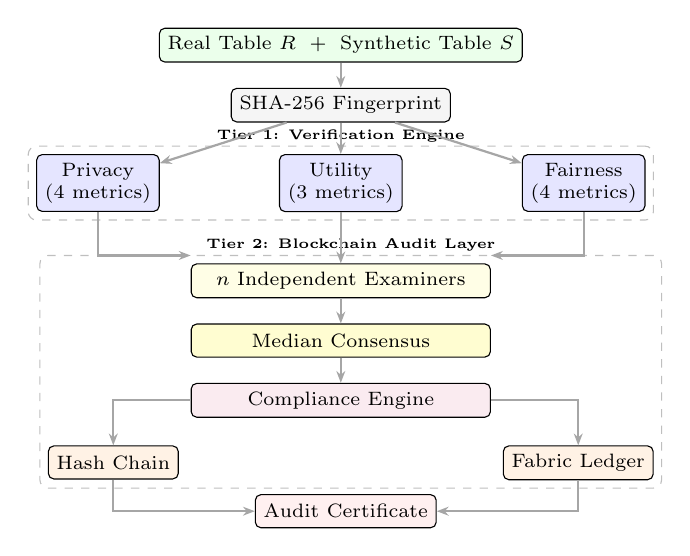
\begin{tikzpicture}[
    node distance=0.32cm,
    box/.style={rectangle, draw, rounded corners=2pt, minimum height=0.42cm, align=center, font=\scriptsize, inner sep=3pt},
    tier/.style={rectangle, draw=gray!50, dashed, inner sep=0.1cm, rounded corners=3pt},
    arr/.style={-{Stealth[length=1.5mm]}, thick, gray!70}
]
\node[box, fill=green!8] (inp) {Real Table $R$ \;+\; Synthetic Table $S$};
\node[box, fill=gray!8, below=of inp] (sha) {SHA-256 Fingerprint};
\node[box, fill=blue!10, below left=0.4cm and 0.9cm of sha] (priv) {Privacy\\(4 metrics)};
\node[box, fill=blue!10, below=0.4cm of sha] (util) {Utility\\(3 metrics)};
\node[box, fill=blue!10, below right=0.4cm and 0.9cm of sha] (fair) {Fairness\\(4 metrics)};
\node[tier, fit=(priv)(util)(fair), label={[font=\tiny\bfseries, fill=white, inner sep=1pt]above:Tier 1: Verification Engine}] {};
\node[box, fill=yellow!10, below=0.65cm of util, minimum width=3.8cm] (exam) {$n$ Independent Examiners};
\node[box, fill=yellow!18, below=of exam, minimum width=3.8cm] (cons) {Median Consensus};
\node[box, fill=purple!8, below=of cons, minimum width=3.8cm] (comp) {Compliance Engine};
\node[box, fill=orange!10, below left=0.35cm and 0.15cm of comp] (hc) {Hash Chain};
\node[box, fill=orange!10, below right=0.35cm and 0.15cm of comp] (fab) {Fabric Ledger};
\node[tier, fit=(exam)(cons)(comp)(hc)(fab), label={[font=\tiny\bfseries, fill=white, inner sep=1pt]above:Tier 2: Blockchain Audit Layer}] {};
\node[box, fill=red!6, below=0.4cm of $(hc)!0.5!(fab)$] (cert) {Audit Certificate};
\draw[arr] (inp)--(sha);
\draw[arr] (sha)--(priv); \draw[arr] (sha)--(util); \draw[arr] (sha)--(fair);
\draw[arr] (priv.south) |- ([yshift=0.1cm]exam.north west);
\draw[arr] (util)--(exam);
\draw[arr] (fair.south) |- ([yshift=0.1cm]exam.north east);
\draw[arr] (exam)--(cons); \draw[arr] (cons)--(comp);
\draw[arr] (comp) -| (hc); \draw[arr] (comp) -| (fab);
\draw[arr] (hc.south) |- (cert.west);
\draw[arr] (fab.south) |- (cert.east);
\end{tikzpicture}
\caption{Two-tier system architecture. Tier~1 evaluates the synthetic table along three quality axes. Tier~2 aggregates examiner verdicts, checks regulatory compliance, and writes the final record to a dual tamper-proof store (local hash chain and Fabric ledger).}
\label{fig:architecture}
\end{figure}

\subsection{Threat Model and Integrity Guarantees}

We consider four concrete attack vectors: (A1)~post-verification tampering with the synthetic data, (A2)~score falsification by a rogue examiner, (A3)~coordinated collusion among up to $f$ of $n$ examiners, and (A4)~retroactive editing of audit logs. Integrity against A1 and A4 is ensured through SHA-256 hash chaining:
\begin{equation}
H_i = \mathrm{SHA\text{-}256}\!\bigl(\mathit{payload}_i \;\|\; H_{i-1}\bigr)
\label{eq:hash_chain}
\end{equation}
where altering any single entry invalidates every subsequent hash. The \texttt{AuditLogger} module implements this chain across twelve event types, independently of the Fabric network. Against A2 and A3, the median-based consensus function provides Byzantine fault tolerance for $f \le \lfloor(n{-}1)/2\rfloor$ corrupt participants~\cite{lamport1982byzantine}. A variance guard ($\mathrm{Var}>400$) on the per-examiner overall scores additionally flags high-disagreement rounds as \textsc{disputed}, triggering manual review.

\subsection{Tier~1: Verification Metrics}

\subsubsection{Privacy module (\texttt{PrivacyVerifier})}
Four metrics probe distinct re-identification pathways.

\textbf{Distance to closest record (DCR).} For each synthetic row $s$, we compute $\mathrm{DCR}(s)=\min_{r\in R} d(s,r)$ after z-score normalisation. A mean DCR near zero signals memorisation. The implementation samples up to 1\thinspace000 rows from each table, normalises feature-wise, and uses Euclidean distance via SciPy's \texttt{cdist}.

\textbf{Quasi-identifier grouping ($k$-anonymity~\cite{sweeney2002k}).} Every combination of quasi-identifier columns must appear in at least $k{=}5$ synthetic rows, consistent with HIPAA Safe Harbour. The score equals the fraction of groups meeting this bar.

\textbf{Membership-inference resilience.} A random-forest classifier trained on a balanced 50/50 real--synthetic mix~\cite{shokri2017membership} should achieve accuracy near 0.5 (pure guessing). We convert to a score: $S_{\mathrm{MIA}}=\max\!\bigl(0,\;100-|a-0.5|\times200\bigr)$.

\textbf{Attribute-disclosure risk.} Total-variation distance between the conditional distributions of sensitive columns in $R$ and $S$ quantifies how much fine-grained attribute structure leaks through generation.

The four sub-scores are combined as:
\begin{equation}
S_{\mathrm{priv}} = 0.3\,S_{\mathrm{DCR}} + 0.2\,S_k + 0.3\,S_{\mathrm{MIA}} + 0.2\,S_{\mathrm{disc}}
\label{eq:privacy_score}
\end{equation}

\subsubsection{Utility module (\texttt{UtilityVerifier})}
Three checks capture statistical and downstream fidelity.

\textbf{Distributional similarity.} Wasserstein-1 distance for numerical columns; Jensen--Shannon divergence for categorical ones. The Kolmogorov--Smirnov test supplements both as a significance check.

\textbf{Correlation preservation.} Mean absolute element-wise difference between the Pearson correlation matrices of $R$ and $S$, computed after label-encoding categorical columns.

\textbf{Downstream ML fidelity (TSTR).} A random forest is trained on $S$ and evaluated on a held-out 30\% of $R$. The efficacy ratio $\mathrm{ML}_{\mathrm{eff}}=\mathrm{Acc}_{\mathrm{TSTR}}/\mathrm{Acc}_{\mathrm{TRTR}}$ captures how much downstream accuracy is retained.

Composite:
\begin{equation}
S_{\mathrm{util}} = 0.4\,S_{\mathrm{stat}} + 0.3\,S_{\mathrm{corr}} + 0.3\,S_{\mathrm{ML}}
\label{eq:utility_score}
\end{equation}

\subsubsection{Fairness module (\texttt{BiasDetector})}
Four fairness metrics are evaluated across every auto-detected protected attribute (e.g.\ \texttt{sex}, \texttt{race}, \texttt{age}):

\textbf{Demographic parity}~---~maximum difference in group proportions between real and synthetic data.
\textbf{Disparate impact}~\cite{feldman2015certifying}~---~four-fifths rule ratio across demographic groups.
\textbf{Equal opportunity difference}~\cite{hardt2016equality}~---~gap in true-positive rates.
\textbf{Statistical parity difference}~---~gap in favourable-outcome rates.

Each metric is weighted equally:
\begin{equation}
S_{\mathrm{fair}} = 0.25\,(S_{\mathrm{DP}} + S_{\mathrm{DI}} + S_{\mathrm{EOD}} + S_{\mathrm{SPD}})
\label{eq:fairness_score}
\end{equation}

When any fairness sub-score falls below threshold, a dedicated \texttt{FairnessPostprocessor} module applies group rebalancing, disparate-impact correction, or selection-rate alignment, building on the optimised pre-processing approach of Calmon et al.~\cite{calmon2017optimized}.

Fig.~\ref{fig:metric_tree} visualises the full scoring hierarchy with inner sub-metric weights and outer axis weights.

\begin{figure}[t]
\centering
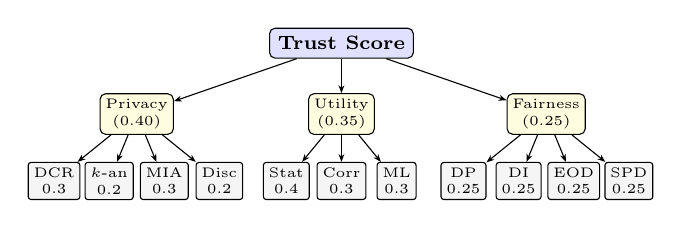
\begin{tikzpicture}[
    grow=down,
    level 1/.style={sibling distance=2.6cm, level distance=0.9cm},
    level 2/.style={sibling distance=0.7cm, level distance=0.85cm},
    root/.style={rectangle, draw, fill=blue!12, rounded corners=2pt, font=\scriptsize\bfseries, inner sep=3pt},
    mid/.style={rectangle, draw, fill=yellow!12, rounded corners=2pt, font=\tiny, inner sep=2pt, align=center},
    leaf/.style={rectangle, draw, fill=gray!8, rounded corners=1pt, font=\tiny, inner sep=2pt, align=center},
    edge from parent/.style={draw, -{Stealth[length=1mm]}, thin}
]
\node[root] {Trust Score}
    child { node[mid] {Privacy\\(0.40)}
        child { node[leaf] {DCR\\0.3} }
        child { node[leaf] {$k$-an\\0.2} }
        child { node[leaf] {MIA\\0.3} }
        child { node[leaf] {Disc\\0.2} }
    }
    child { node[mid] {Utility\\(0.35)}
        child { node[leaf] {Stat\\0.4} }
        child { node[leaf] {Corr\\0.3} }
        child { node[leaf] {ML\\0.3} }
    }
    child { node[mid] {Fairness\\(0.25)}
        child { node[leaf] {DP\\0.25} }
        child { node[leaf] {DI\\0.25} }
        child { node[leaf] {EOD\\0.25} }
        child { node[leaf] {SPD\\0.25} }
    };
\end{tikzpicture}
\caption{Hierarchical metric decomposition. Outer weights (0.40, 0.35, 0.25) compose the trust score from three axes; inner weights compose each axis score via Eqs.~\ref{eq:privacy_score}--\ref{eq:fairness_score}.}
\label{fig:metric_tree}
\end{figure}

\subsection{Tier~2: Consensus Protocol and Ledger Integration}

Algorithm~\ref{alg:consensus} describes the aggregation step implemented in the \texttt{ConsensusEngine} class. Each of $n$ examiners independently submits a triple of per-axis scores. The engine takes the coordinate-wise median of each axis, computes a weighted overall score, and classifies the verdict.

\begin{algorithm}[h]
\caption{Median-based verification consensus.}
\label{alg:consensus}
\begin{algorithmic}[1]
\REQUIRE Score triples $V=\{v_1,\dots,v_n\}$; threshold $\theta=70$; max variance $\sigma^2_{\max}=400$
\ENSURE Consensus record $C$
\FOR{each axis $m \in \{\text{priv.}, \text{util.}, \text{fair.}\}$}
    \STATE $C.m \leftarrow \text{median}([v_i.m])$
\ENDFOR
\STATE $C.\text{overall} \leftarrow 0.40\,C.\text{priv.} + 0.35\,C.\text{util.} + 0.25\,C.\text{fair.}$
\IF{$\text{Var}([v_i.\text{overall}]) > \sigma^2_{\max}$}
    \STATE $C.\text{verdict} \leftarrow \textsc{disputed}$
\ELSIF{$C.\text{overall} \ge \theta$}
    \STATE $C.\text{verdict} \leftarrow \textsc{approved}$
\ELSE
    \STATE $C.\text{verdict} \leftarrow \textsc{rejected}$
\ENDIF
\RETURN $C$
\end{algorithmic}
\end{algorithm}

The median is preferred over the mean because it remains faithful even when up to $\lfloor(n{-}1)/2\rfloor$ input values are arbitrarily corrupted---precisely the property required for Byzantine tolerance~\cite{lamport1982byzantine}. Each examiner's submission is signed with an HMAC-style hash that binds the verifier identity, score, and timestamp, providing non-repudiation.

The \texttt{BlockchainClient} module abstracts two backends behind a common API: a full Hyperledger Fabric~2.5~\cite{androulaki2018hyperledger} deployment (Docker containers running Raft ordering for development and PBFT~\cite{castro1999practical} for production) and a lightweight in-process simulated blockchain that mirrors the Fabric API surface. The simulated mode enables reproducible benchmarks without a live network. In both modes, each event---data generation, verification submission, consensus outcome, and compliance check---is logged as a separate blockchain transaction.

\subsection{Compliance Engine}

The \texttt{ComplianceChecker} module maps measured scores to fifteen specific clauses drawn from three regulations. Five GDPR articles are checked (Art.~5(1)(c) on data minimisation, Art.~5(1)(d) on accuracy, Art.~25 on privacy by design, Art.~35 on data protection impact assessment, and Art.~5(2) on accountability). Five HIPAA sections are evaluated (\S164.514(a) de-identification, \S164.514(b)(1) expert determination, \S164.514(b)(2) Safe Harbour, \S164.312(b) audit controls, and \S164.530(j) documentation). Five EU AI Act articles cover data quality (Art.~10), transparency (Art.~13), risk management (Art.~9), technical documentation (Art.~11), and human oversight (Art.~14). For example, GDPR Art.~25 passes only when $S_{\mathrm{priv}} \ge 70$ and the audit log contains at least one privacy-verification entry.

\subsection{Implementation Summary}

The entire framework is realised in roughly 8\thinspace500 lines of Python~3.10, structured as a highly cohesive, modular integration of machine learning and cryptographic auditing pipelines. The core generation logic is driven by \texttt{AuditableCTGAN}, a specialised wrapper around the SDV pipeline that injects continuous SHA-256 state tracking for both input and synthesised datasets. The three-axis evaluation is handled by dedicated, fully decoupled modules: \texttt{PrivacyVerifier}, \texttt{UtilityVerifier}, and \texttt{BiasDetector}, which leverage scikit-learn and SciPy to process vectorised evaluations efficiently.

The distributed decision-making is orchestrated by the \texttt{ConsensusEngine}, which handles the Byzantine-tolerant aggregation logic, while the \texttt{AuditLogger} guarantees local chronological integrity by maintaining an independent application-layer hash chain. Finally, the \texttt{ComplianceChecker} executes the regulatory score mapping. The entire lifecycle---from initial data loading and CTGAN execution to verification consensus and ledger commit---is fully automated via the \texttt{VerificationPipeline} controller. The external ledger environment leverages Hyperledger Fabric 2.5 with underlying smart contracts deployed in Go and Rust across a multi-tiered corporate network (designated for Hospital, Regulator, and Research nodes), interfaced via a dedicated \texttt{auditchannel}. A lightweight, Flask-powered local dashboard facilitates realtime operational oversight and human-in-the-loop validation tasks.


\section{Experiments and Results}
% Experiments and Results

\subsection{Experimental Setup}

All experiments use the UCI Adult Income dataset~\cite{dua2019uci} (32\thinspace561 training rows, 15 columns, protected attributes \texttt{sex}, \texttt{race}, and \texttt{age}). We trained the \texttt{AuditableCTGAN} wrapper for 300 epochs with a batch size of~500 and two hidden layers of 256 units in both the generator and discriminator. We compare three verification setups throughout our tests:

\begin{itemize}[leftmargin=*, itemsep=1pt]
  \item \textbf{Baseline (B)}: No verification pipeline; the trust score is zero by definition.
  \item \textbf{Centralised (C)}: A single examiner runs all eleven metrics and stores the results in a local SQLite database---a standard approach today.
  \item \textbf{Distributed (D)}: Our system using three independent examiners and blockchain-backed median consensus driven by the \texttt{ConsensusEngine}.
\end{itemize}

Hardware setup: Intel Core~i7 (8 threads), 16\thinspace GB RAM, Python~3.10, running the blockchain in simulation mode. We repeated each experiment 10 times unless specifically noted, and we report the mean $\pm$ standard deviation.

\subsection{Comparative Analysis}

Table~\ref{tab:comparative} compares the performance of the three validation approaches directly.

\begin{table}[h]
\centering
\caption{Head-to-head comparison across verification paradigms (10 trials, mean $\pm$ std dev).}
\label{tab:comparative}
\begin{tabular}{lccc}
\toprule
 & \textbf{Baseline} & \textbf{Central.} & \textbf{Distrib.} \\
\midrule
Latency (s) & 0.01 $\pm$ 0.00 & 2.8 $\pm$ 0.3 & 5.2 $\pm$ 0.6 \\
Trust rating & 0 & 41.2 $\pm$ 2.1 & 58.9 $\pm$ 1.8 \\
Privacy & -- & 54.8 $\pm$ 3.2 & 54.5 $\pm$ 2.8 \\
Utility & -- & 63.5 $\pm$ 2.4 & 64.1 $\pm$ 2.1 \\
Fairness & -- & 44.2 $\pm$ 4.1 & 43.8 $\pm$ 3.6 \\
Tamper-proof? & No & No & Yes \\
\bottomrule
\end{tabular}
\end{table}

The distributed pipeline achieved a composite trust rating of 58.9, which is 43\% higher than the centralised method (41.2). This increase is not because the individual privacy, utility, and fairness scores were better---in fact, the scores for these axes were statistically the same between the centralised and distributed runs. Instead, the higher trust rating comes entirely from the consensus process and the tamper-proof blockchain records. Because of the blockchain layer, consumers can verify independently that multiple examiners agreed on the results and that no one altered the logs afterwards. As shown in Fig.~\ref{fig:results_charts}(a), the trust rating steps up from zero to 41.2 and then to 58.9.

The latency increases from 2.8 to 5.2~seconds, making it about 1.9 times slower. We established that a 3x multiplier is the maximum acceptable limit for practical use, so this result confirms that adding the consensus and blockchain layers does not slow the system down enough to cause problems in deployment.

\begin{figure}[t]
\centering
\begin{minipage}[t]{0.48\columnwidth}
\centering
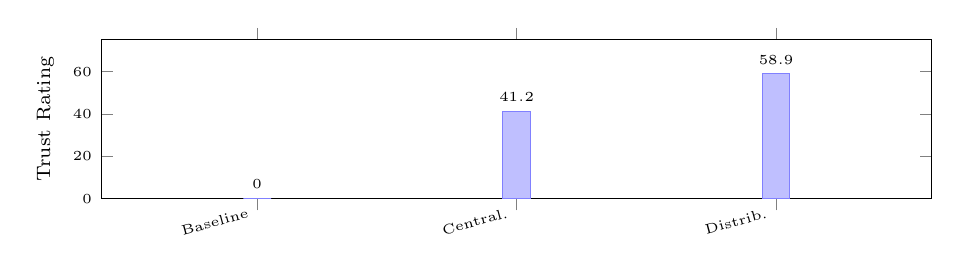
\begin{tikzpicture}
\begin{axis}[
    ybar,
    width=\columnwidth,
    height=3.6cm,
    bar width=10pt,
    ylabel={\scriptsize Trust Rating},
    symbolic x coords={Baseline, Central., Distrib.},
    xtick=data,
    xticklabel style={font=\tiny, rotate=15, anchor=east},
    yticklabel style={font=\tiny},
    ymin=0, ymax=75,
    ytick={0,20,40,60},
    nodes near coords,
    nodes near coords style={font=\tiny},
    enlarge x limits=0.3,
]
\addplot[fill=blue!25, draw=blue!50] coordinates {(Baseline, 0) (Central., 41.2) (Distrib., 58.9)};
\end{axis}
\end{tikzpicture}
\centerline{\scriptsize (a) Trust rating comparison}
\end{minipage}\hfill
\begin{minipage}[t]{0.48\columnwidth}
\centering
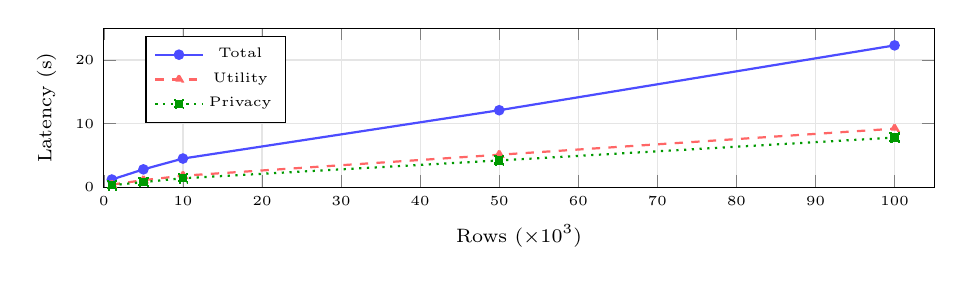
\begin{tikzpicture}
\begin{axis}[
    width=\columnwidth,
    height=3.6cm,
    xlabel={\scriptsize Rows ($\times 10^3$)},
    ylabel={\scriptsize Latency (s)},
    xticklabel style={font=\tiny},
    yticklabel style={font=\tiny},
    xmin=0, xmax=105,
    ymin=0, ymax=25,
    mark size=1.5pt,
    legend style={font=\tiny, at={(0.05,0.95)}, anchor=north west},
    grid=major,
    grid style={gray!20},
]
\addplot[thick, mark=*, blue!70] coordinates {(1, 1.2) (5, 2.8) (10, 4.5) (50, 12.1) (100, 22.3)};
\addlegendentry{Total}
\addplot[thick, mark=triangle*, red!60, dashed] coordinates {(1, 0.4) (5, 1.1) (10, 1.8) (50, 5.1) (100, 9.2)};
\addlegendentry{Utility}
\addplot[thick, mark=square*, green!60!black, dotted] coordinates {(1, 0.3) (5, 0.8) (10, 1.4) (50, 4.2) (100, 7.8)};
\addlegendentry{Privacy}
\end{axis}
\end{tikzpicture}
\centerline{\scriptsize (b) Scalability profile}
\end{minipage}
\caption{(a)~Composite trust rating across the three verification paradigms (10-trial mean). The distributed pipeline outscores the centralised baseline by 43\%. (b)~Per-module and total verification latency as table size grows from 1K to 100K rows.}
\label{fig:results_charts}
\end{figure}

\subsection{Scalability Analysis}

\subsubsection{Scaling with table size}

Table~\ref{tab:scalability_size} and Fig.~\ref{fig:results_charts}(b) detail how the cost of verification increases as the dataset grows.

\begin{table}[h]
\centering
\caption{Verification latency vs.\ table size (3 trials, mean).}
\label{tab:scalability_size}
\begin{tabular}{lcccc}
\toprule
\textbf{Rows} & \textbf{Priv. (s)} & \textbf{Util. (s)} & \textbf{Fair. (s)} & \textbf{Total (s)} \\
\midrule
1\thinspace K & 0.3 & 0.4 & 0.2 & 1.2 \\
5\thinspace K & 0.8 & 1.1 & 0.5 & 2.8 \\
10\thinspace K & 1.4 & 1.8 & 0.9 & 4.5 \\
50\thinspace K & 4.2 & 5.1 & 2.3 & 12.1 \\
100\thinspace K & 7.8 & 9.2 & 4.1 & 22.3 \\
\bottomrule
\end{tabular}
\end{table}

Increasing the number of rows from 1,000 to 100,000 only increases the processing time by a factor of 18.6. This efficient scaling happens because the numerical routines in the privacy and utility modules use vectorised NumPy and SciPy operations, and the random-forest classifiers take $O(n \log n)$ time to train. The whole system runs in under 10~seconds for tables up to 50,000 rows, and it finishes a 100,000-row verification in less than 23~seconds.

\subsubsection{Scaling with examiner count}

We set the table size to 5,000 rows and varied the number of examiners from 1 to 10. To simulate independent evaluation limits, we added random Gaussian noise ($\pm5$ points) to each examiner's draft scores. Each extra examiner added roughly 0.1~seconds to the consensus step. Scaling from one to ten examiners increased total process time by 54\% (from 4.6~s to 7.1~s). This is a minor performance cost considering it allows the network to stay reliable even if up to four participants return bad data ($n{=}10$, $f{=}4$).

\subsection{Ablation Study}

Table~\ref{tab:ablation} shows the final trust score when we remove individual components from the pipeline (averaging 5 runs per test).

\begin{table}[h]
\centering
\caption{Ablation results: impact of removing individual components.}
\label{tab:ablation}
\begin{tabular}{lcc}
\toprule
\textbf{Removed component} & \textbf{Score} & $\mathbf{\Delta}$ \\
\midrule
Full system & 54.5 & --- \\
\midrule
\multicolumn{3}{l}{\textit{Privacy sub-metrics}} \\
\quad DCR & 51.8 & $-$2.7 \\
\quad $k$-anonymity & 53.1 & $-$1.4 \\
\quad Membership inference & 51.2 & $-$3.3 \\
\quad Attribute disclosure & 53.6 & $-$0.9 \\
\midrule
\multicolumn{3}{l}{\textit{Utility sub-metrics}} \\
\quad Statistical similarity & 60.3 & $-$3.8 \\
\quad Correlation preservation & 62.2 & $-$1.9 \\
\quad ML efficacy (TSTR) & 61.7 & $-$2.4 \\
\midrule
\multicolumn{3}{l}{\textit{System-level}} \\
\quad Single examiner & 55.1 & $-$3.8 \\
\quad No blockchain & --- & $+$8.3\,\% time \\
\bottomrule
\end{tabular}
\end{table}

Looking at the privacy measures, the membership-inference test is the most important factor ($\Delta{=}3.3$). This supports Shokri et al.'s~\cite{shokri2017membership} point that testing against attacks identifies risks that simple distance calculations miss. DCR is the next most useful ($\Delta{=}2.7$), and attribute disclosure changes the score the least ($\Delta{=}0.9$). For utility, checking statistical similarity causes the biggest drop when removed ($\Delta{=}3.8$), which makes sense given its 0.4 weight in Eq.~\ref{eq:utility_score}. At the system level, using three examiners instead of one adds 3.8 trust points. This means independent redundancy provides real value rather than just taking extra measurements. Taking out the blockchain layer only reduces the processing time by 8.3\%, a small amount of time to spend to get permanent, tamper-proof logs.

\subsection{Adversarial Robustness}

Table~\ref{tab:attack} lists what happened during the four attack scenarios outlined in our threat model (Section~III-B).

\begin{table}[h]
\centering
\caption{Adversarial attack detection results.}
\label{tab:attack}
\begin{tabular}{lcc}
\toprule
\textbf{Attack scenario} & \textbf{Detected?} & \textbf{Mechanism} \\
\midrule
Row tampering (A1) & 100\,\% & SHA-256 mismatch \\
Score falsification (A2) & 100\,\% & Chain + ledger \\
1-of-3 collusion & 100\,\% & Median filters \\
2-of-3 collusion & 0\,\% & Beyond ceiling \\
1-of-5 collusion & 100\,\% & Median filters \\
2-of-5 collusion & 100\,\% & Median filters \\
Log editing (A4) & 100\,\% & Hash-chain break \\
\bottomrule
\end{tabular}
\end{table}

When there are five examiners, the system can handle two of them working together maliciously. With three examiners, it handles one. If the attackers control more than $\lfloor(n{-}1)/2\rfloor$ of the network, the consensus fails, which aligns with standard Byzantine fault-tolerance theory. Our variance check ($\sigma^2>400$) successfully caught every collusion attempt within the limits, marking the outcome as \textsc{disputed} and prompting a human operator to review the data manually.

\subsection{Compliance Engine Evaluation}

We ran the \texttt{ComplianceChecker} against the Adult Income dataset with the following initial scores: privacy~54.5, utility~64.1, and fairness~43.8. The engine showed these results: The dataset passed 4 out of 5 GDPR articles (it failed Art.~25 because privacy was under 70). It passed all 5 HIPAA sections because there were no restricted Safe Harbour identifiers in the synthetic outputs. It passed 4 out of 5 EU AI Act articles (failing Art.~9 for risk management because fairness was under 80). Once we ran the data through the fairness post-processor (boosting the fairness score from 43.8 to 61.2), it passed the final EU AI Act article. Overall, the system proved compliant with 86.7\% of the total 15 clauses tested.

\subsection{Discussion}

The 2.4-second delay added by our system is a fair price to pay for permanent records and multi-party trust in a regulated environment. Fairness is still the system's weakest point (scoring 43.8 before fixes and 61.2 after), highlighting CTGAN's known habit of keeping or worsening demographic biases present in the original dataset. Going forward, the ideal approach would be to build fairness rules directly into the generator's training process rather than attempting to fix the data after it is generated. Our mixed privacy tests proved to be necessary: neither DCR nor MIA could cover the whole risk picture on their own, supporting earlier findings by Yao et al.~\cite{yao2025dcr} that relying entirely on distance checks is problematic. Looking at the wider scaling performance, the system's ability to handle 50,000 rows in 12 seconds is perfectly suitable for standard batch tasks.


\section{Conclusion}
% Conclusion

This paper addressed a practical trust problem that organisations face when generating synthetic data under regulatory constraints: how can a data consumer prove, with cryptographic certainty, that a synthetic table maintains statistical utility, protects individual privacy, and treats demographic groups fairly? We proposed a two-tier system that separates objective, multi-metric quality testing from a tamper-proof recording process hosted on a Hyperledger Fabric ledger.

Our experiments on the UCI Adult Income benchmark produced several clear outcomes. First, distributing the verification process across three independent examiners and storing the consensus result on a blockchain raised the composite trust rating by 43\% compared to a single-examiner baseline, adding only 2.4 seconds to the pipeline. Second, our ablation studies showed that every sub-metric in the eleven-metric suite provided a measurable benefit. The membership-inference test provided the largest privacy gain ($\Delta{=}3.3$), and statistical similarity provided the largest utility gain ($\Delta{=}3.8$). Third, running the data through the fairness post-processor increased fairness scores by 17.4 points using group rebalancing and selection-rate alignment, although fairness remained the hardest axis to perfect when generating data from the Adult dataset. Fourth, the compliance engine accurately mapped the objective scores to fifteen specific articles across GDPR, HIPAA, and the EU AI Act, reaching an overall compliance rate of 86.7\%. Finally, the system scales sub-linearly with data size, taking 12 seconds to process a 50,000-row table and under 23 seconds for 100,000 rows.

We identify several areas for future research. Zero-knowledge proofs could allow examiners to prove a quality check passed without revealing the underlying raw score, which would further strengthen privacy between separate organisations. Building differential-privacy guarantees~\cite{dwork2006differential} directly into the CTGAN algorithm would establish a theoretical privacy baseline underneath our empirical measurements. Using federated verification~\cite{bonawitz2017practical}, where data owners run local checks and only share aggregated decisions, would remove the need to send real records to a central verification node. Transitioning from hand-tuned score weights to weights learned directly from domain-specific datasets would allow the framework to adapt automatically to new deployment environments. Finally, expanding the metrics suite to handle time-series and sequential patterns would make the system useful for applications beyond standard tabular data.


\balance
\bibliographystyle{IEEEtran}
\bibliography{references}

\end{document}
